\subsection{Trigger}
\subsubsection{Nhóm Trigger 1}

\textbf{Mô tả Triggers:} Nhóm Triggers 1 dùng để tính toán, cập nhật số lượng nhân viên có trong một phòng ban.

\textbf{Câu lệnh tạo Triggers}
\begin{minted}{mysql}
-- Trigger sau khi thêm nhân viên
CREATE TRIGGER update_employee_count_after_insert 
AFTER INSERT ON NhanVien
FOR EACH ROW
BEGIN
    UPDATE PhongBan 
    SET SoLuongNhanVien = SoLuongNhanVien + 1
    WHERE MaPhongBan = NEW.MaPhongBan;
END //
-- Trigger sau khi cập nhật nhân viên
CREATE TRIGGER update_employee_count_after_update
AFTER UPDATE ON NhanVien
FOR EACH ROW
BEGIN
    -- Nếu phòng ban của nhân viên thay đổi, cập nhật số lượng nhân viên ở phòng ban cũ và mới
    IF OLD.MaPhongBan != NEW.MaPhongBan THEN
        -- Giảm số lượng nhân viên ở phòng ban cũ
        UPDATE PhongBan
        SET SoLuongNhanVien = SoLuongNhanVien - 1
        WHERE MaPhongBan = OLD.MaPhongBan;
        
        -- Tăng số lượng nhân viên ở phòng ban mới
        UPDATE PhongBan
        SET SoLuongNhanVien = SoLuongNhanVien + 1
        WHERE MaPhongBan = NEW.MaPhongBan;
    END IF;
END//
-- Trigger sau khi xóa nhân viên
CREATE TRIGGER update_employee_count_after_delete
AFTER DELETE ON NhanVien
FOR EACH ROW
BEGIN
    UPDATE PhongBan 
    SET SoLuongNhanVien = SoLuongNhanVien - 1
    WHERE MaPhongBan = OLD.MaPhongBan;
END //
\end{minted}

\newpage
\textbf{Kiểm tra Trigger}
\begin{itemize}
    \item [--] Kiểm tra thao tác thêm nhân viên: Thêm 3 nhân viên mới vào phòng ban có mã phòng ban là 'PB0101'
    \begin{figure}[H]
        \centering
        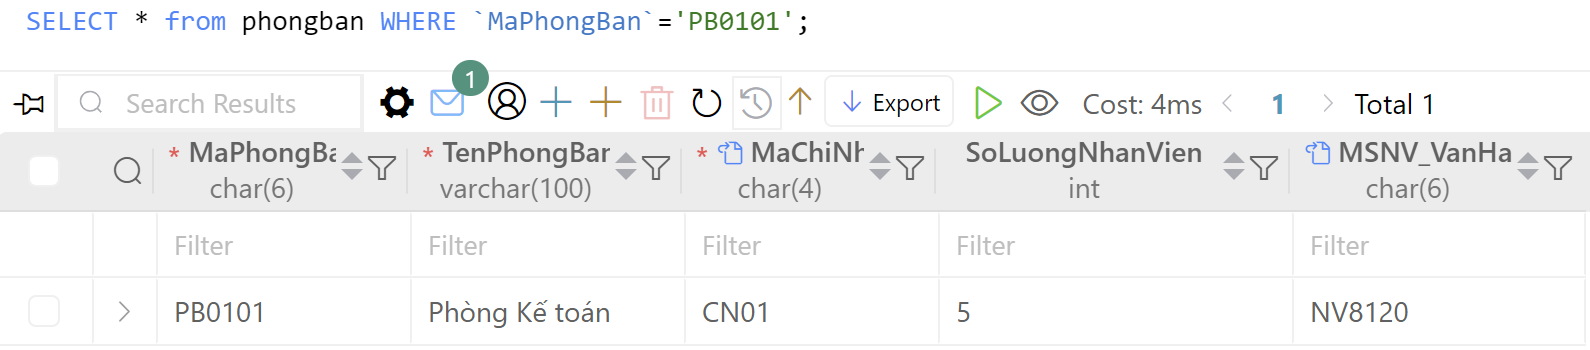
\includegraphics[width=\linewidth]{content/images/trigger_1_1.png}
        \caption{Thông tin của phòng ban 'PB0101' ban đầu, số nhân viên hiện tại là 5}
        \label{fig:trigger_1_1}
    \end{figure}
    \begin{figure}[H]
        \centering
        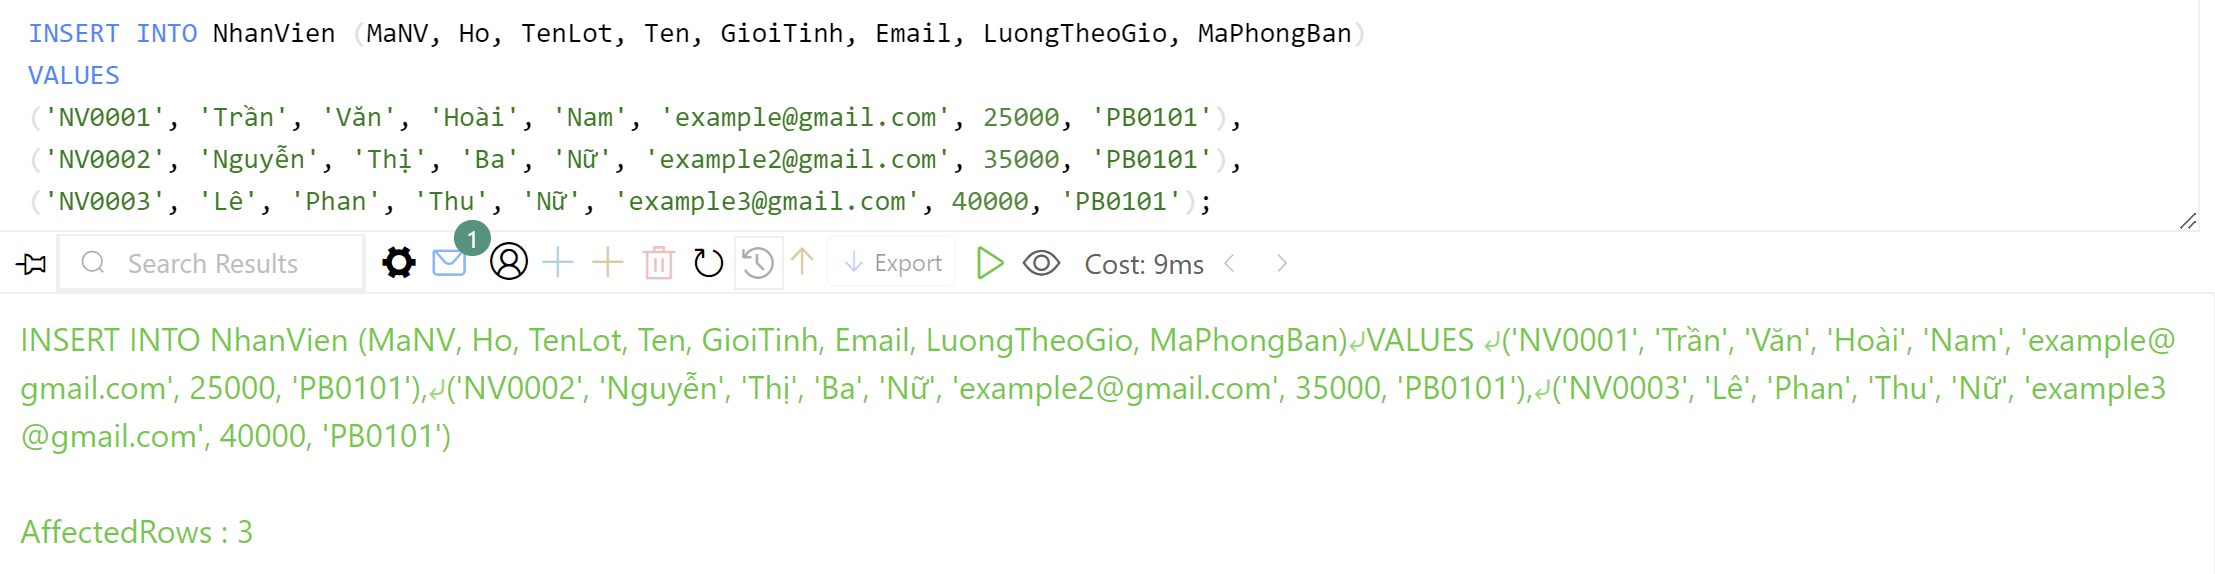
\includegraphics[width=\linewidth]{content/images/trigger_1_2.png}
        \caption{Thực hiện thêm 3 nhân viên vào phòng ban 'PB0101'}
        \label{fig:trigger_1_2}
    \end{figure}
    \begin{figure}[H]
        \centering
        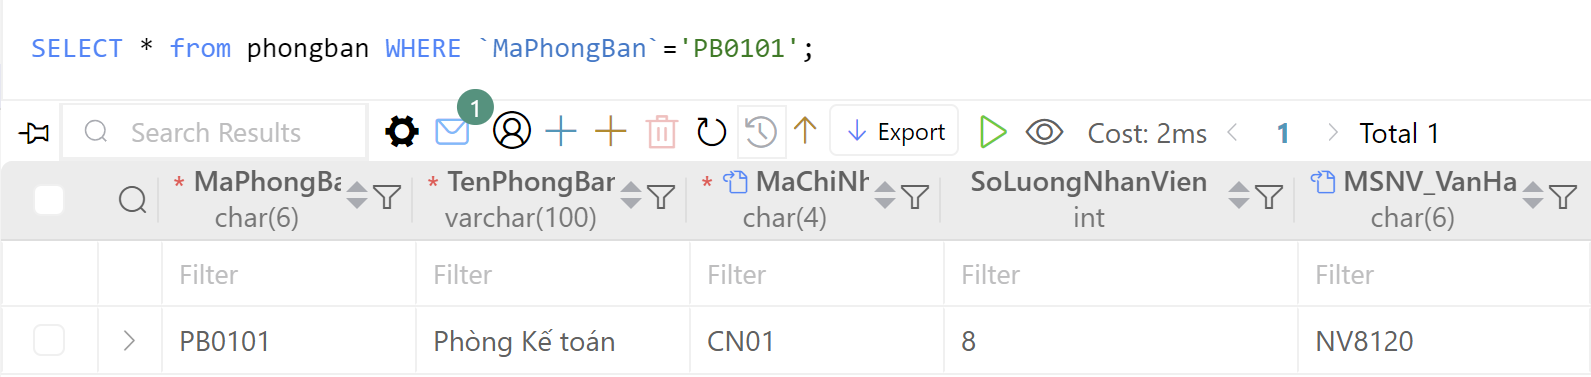
\includegraphics[width=\linewidth]{content/images/trigger_1_3.png}
        \caption{Thông tin của phòng ban 'PB0101', số nhân viên đã tăng từ 5 lên 8}
        \label{fig:trigger_1_3}
    \end{figure}
    \item [--] Kiểm tra sau thao tác cập nhật thông tin về phòng ban của nhân viên: Chuyển 2 nhân viên đang trong phòng ban 'PB0101' sang phòng ban 'PB0201'
    \begin{figure}[H]
        \centering
        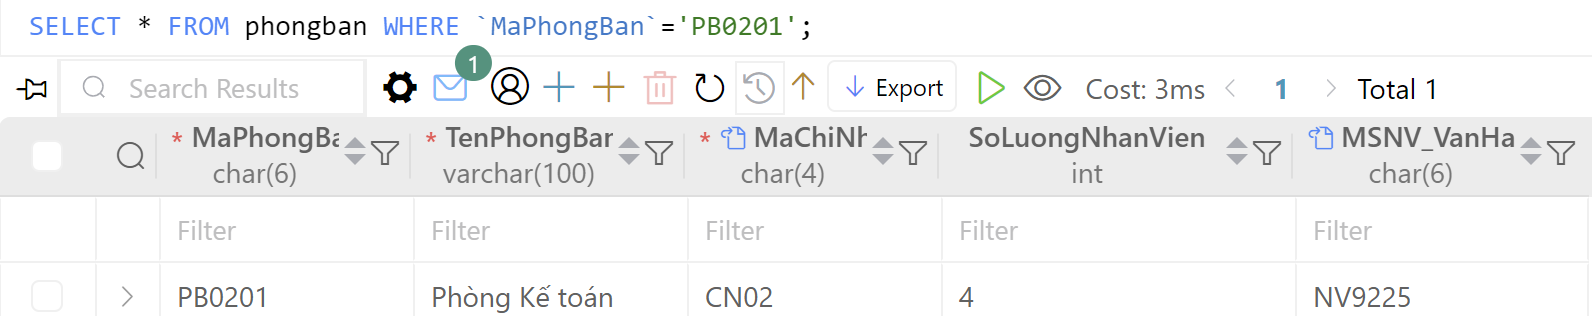
\includegraphics[width=\linewidth]{content/images/trigger_1_4.png}
        \caption{Thông tin của phòng ban 'PB0201' ban đầu, số nhân viên hiện tại là 4}
        \label{fig:trigger_1_4}
    \end{figure}
    \begin{figure}[H]
        \centering
        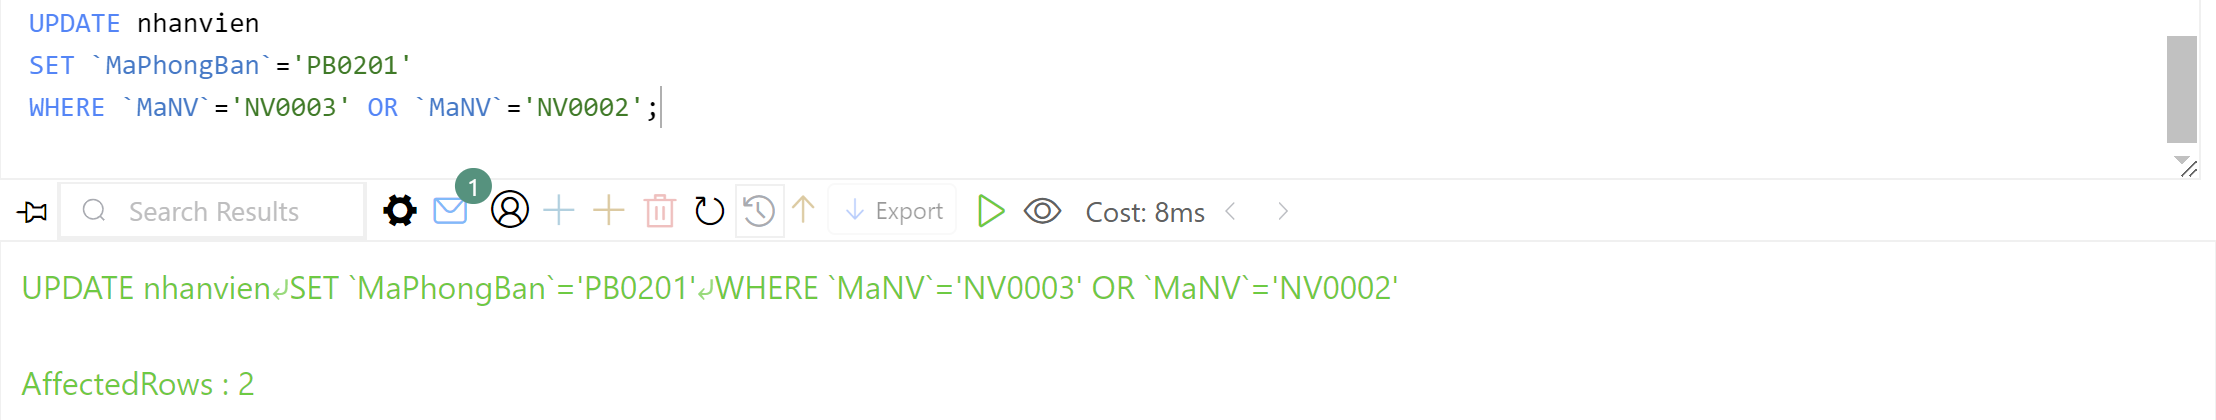
\includegraphics[width=\linewidth]{content/images/trigger_1_5.png}
        \caption{Thực hiện việc chuyển hai nhân viên từ phòng ban 'PB0101' sang phòng ban 'PB0201'}
        \label{fig:trigger_1_5}
    \end{figure}
    \begin{figure}[H]
        \centering
        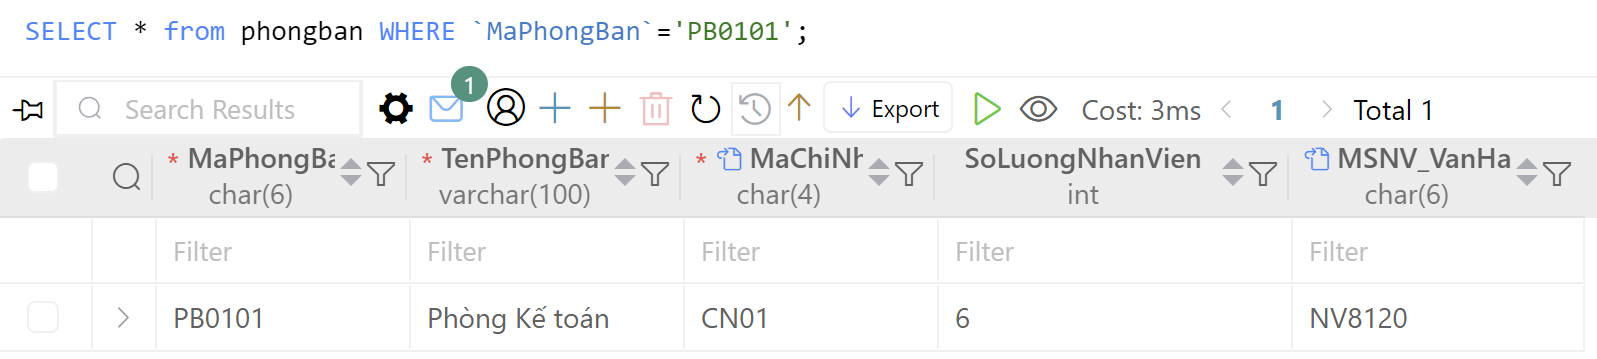
\includegraphics[width=\linewidth]{content/images/trigger_1_6.png}
        \caption{Thông tin của phòng ban 'PB0101', số nhân viên đã giảm từ 8 xuống 6}
        \label{fig:trigger_1_6}
    \end{figure}
    \begin{figure}[H]
        \centering
        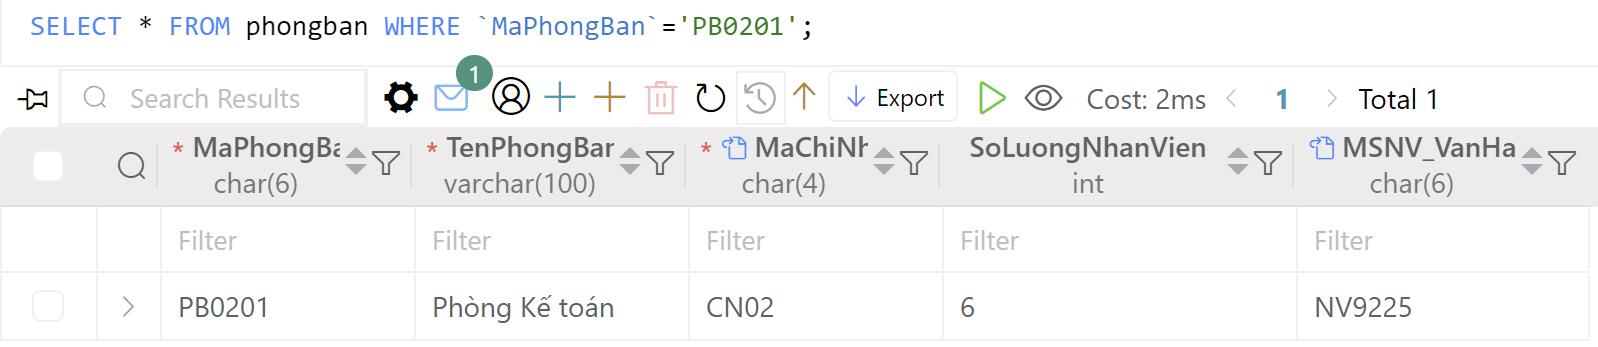
\includegraphics[width=\linewidth]{content/images/trigger_1_7.png}
        \caption{Thông tin của phòng ban 'PB0201', số nhân viên đã tăng từ 4 lên 6}
        \label{fig:trigger_1_7}
    \end{figure}
    \item [--] Kiểm tra sau thao tác xóa nhân viên: Xóa 1 nhân viên từ phòng ban 'PB0201'
    \begin{figure}[H]
        \centering
        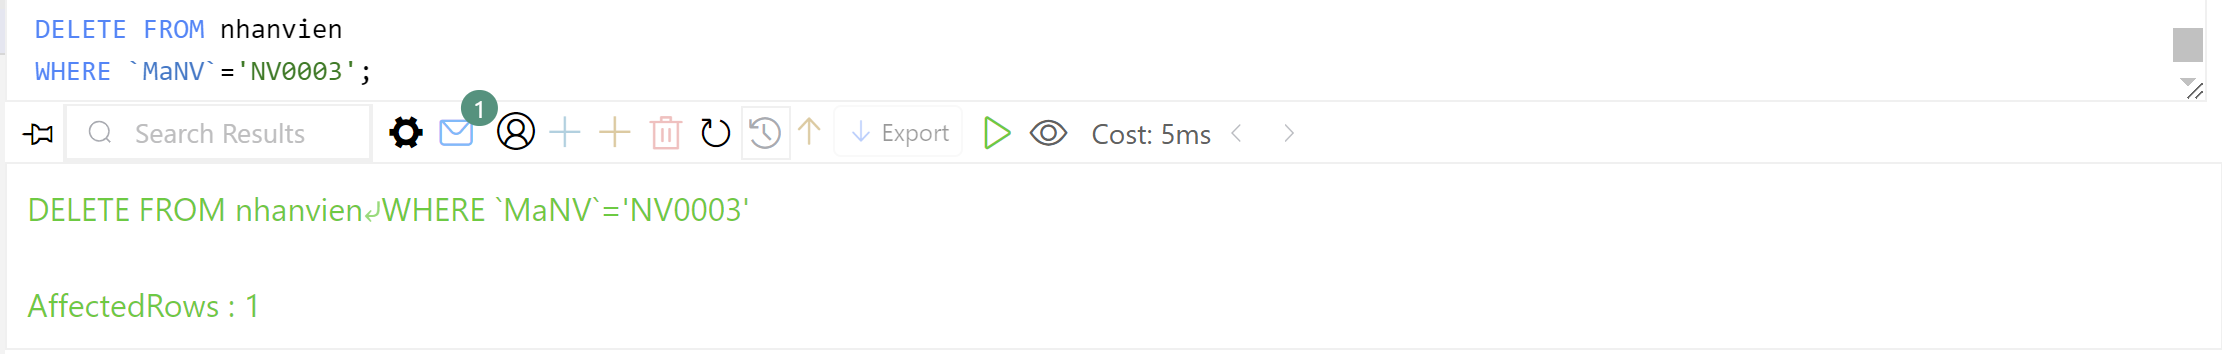
\includegraphics[width=\linewidth]{content/images/trigger_1_8.png}
        \caption{Thực hiện việc xóa một nhân viên thuộc phòng ban 'PB0201'}
        \label{fig:trigger_1_8}
    \end{figure}
    \begin{figure}[H]
        \centering
        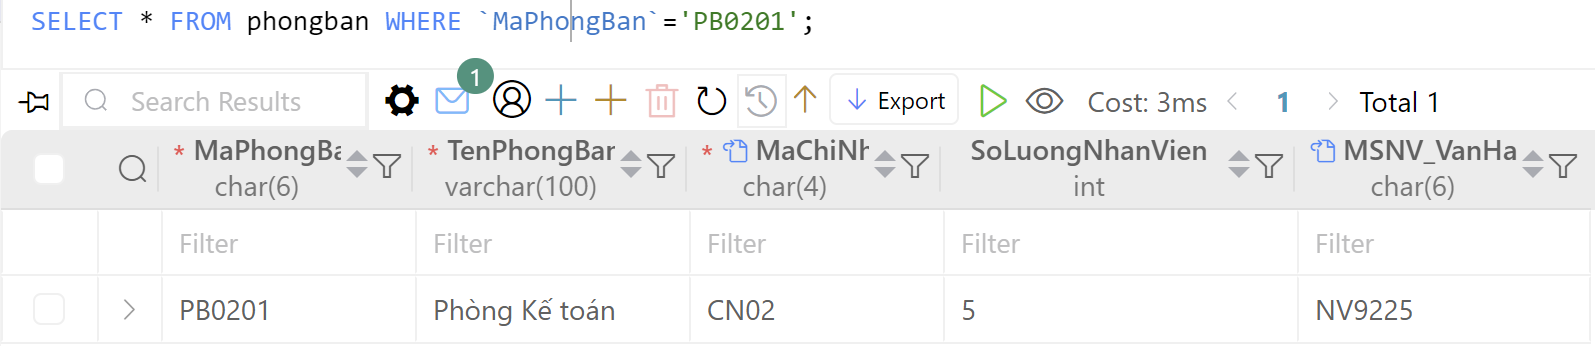
\includegraphics[width=\linewidth]{content/images/trigger_1_9.png}
        \caption{Thông tin của phòng ban 'PB0201', số nhân viên đã giảm từ 6 xuống 5}
        \label{fig:trigger_1_9}
    \end{figure}
\end{itemize}

\newpage
\subsubsection{Nhóm Trigger 2}
\textbf{Mô tả Triggers:} Nhóm Triggers 2 dùng để tính toán tổng số giờ làm việc trong ngày của một nhân viên khi họ thực hiện việc chấm công.

\textbf{Câu lệnh tạo Triggers}
\begin{minted}{mysql}
CREATE TRIGGER update_total_hours_after_insert
AFTER INSERT ON LanRaVao
FOR EACH ROW
BEGIN
    DECLARE total_hours DECIMAL(5, 2);
    SET total_hours = TIMESTAMPDIFF(MINUTE, NEW.GioVao, NEW.GioRa) / 60;
    
    UPDATE BangChamCong
    SET TongSoGioLam = COALESCE(TongSoGioLam, 0) + total_hours
    WHERE MaNV = NEW.MaNV AND Ngay = NEW.Ngay;
END //

CREATE TRIGGER update_total_hours_after_update
AFTER UPDATE ON LanRaVao
FOR EACH ROW
BEGIN
    DECLARE total_hours DECIMAL(5, 2);
    DECLARE previous_hours DECIMAL(5, 2);
    SET previous_hours = TIMESTAMPDIFF(MINUTE, OLD.GioVao, OLD.GioRa) / 60;
    SET total_hours = TIMESTAMPDIFF(MINUTE, NEW.GioVao, NEW.GioRa) / 60;
    UPDATE BangChamCong
    SET TongSoGioLam = COALESCE(TongSoGioLam, 0) + total_hours - previous_hours
    WHERE MaNV = NEW.MaNV AND Ngay = NEW.Ngay;
END;

CREATE TRIGGER update_total_hours_after_delete
AFTER DELETE ON LanRaVao
FOR EACH ROW
BEGIN
    DECLARE total_hours DECIMAL(5, 2);
    SET total_hours = TIMESTAMPDIFF(MINUTE, OLD.GioVao, OLD.GioRa) / 60;
    
    UPDATE BangChamCong
    SET TongSoGioLam = COALESCE(TongSoGioLam, 0) - total_hours
    WHERE MaNV = OLD.MaNV AND Ngay = OLD.Ngay;
END //    
\end{minted}

\newpage
\textbf{Kiểm tra Trigger}: Quan sát giá trị của thuộc tính TongSoGioLam trong bảng BangChamCong của nhân viên 'NV0001' trong ngày 13/12/2024 khi thực hiện các thao tác thêm, sửa và xóa trong bảng LanRaVao.
\begin{itemize}
    \item [--] Kiểm tra thao tác thêm lần ra vào
    \begin{figure}[H]
        \centering
        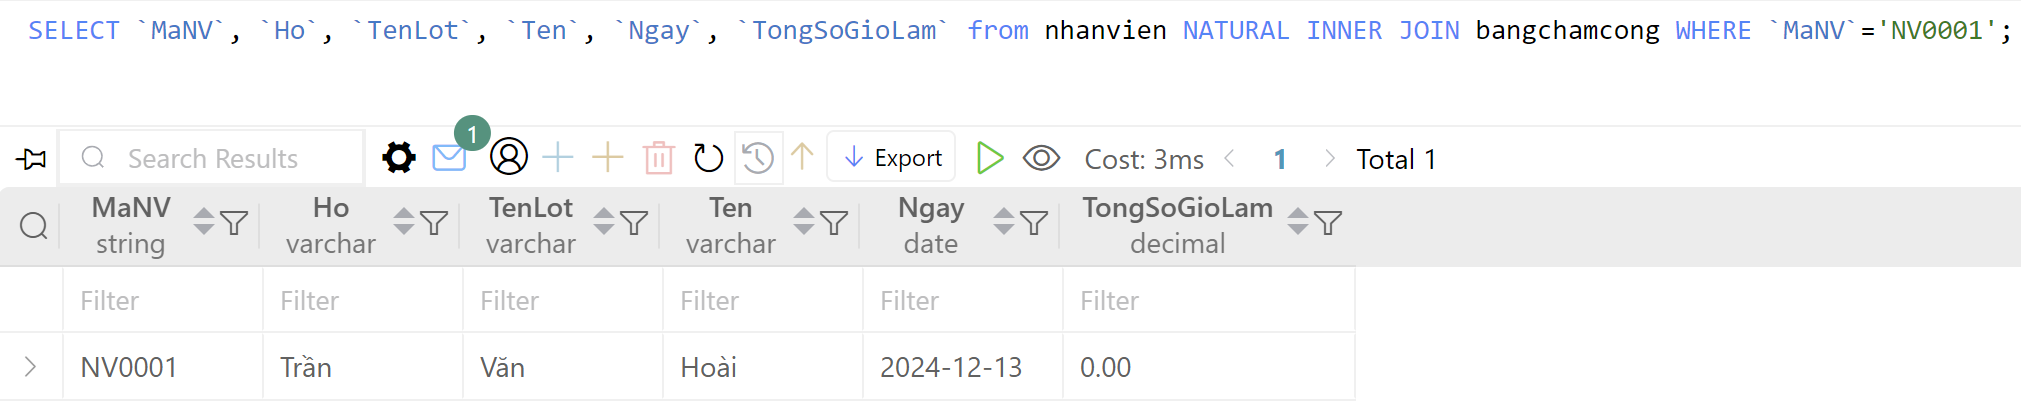
\includegraphics[width=\linewidth]{content/images/trigger_2_1.png}
        \caption{Thông tin ban đầu của nhân viên 'NV0001', với tổng số giờ làm trong ngày 13/12/2024 là 0}
        \label{fig:trigger_2_1}
    \end{figure}
    \begin{figure}[H]
        \centering
        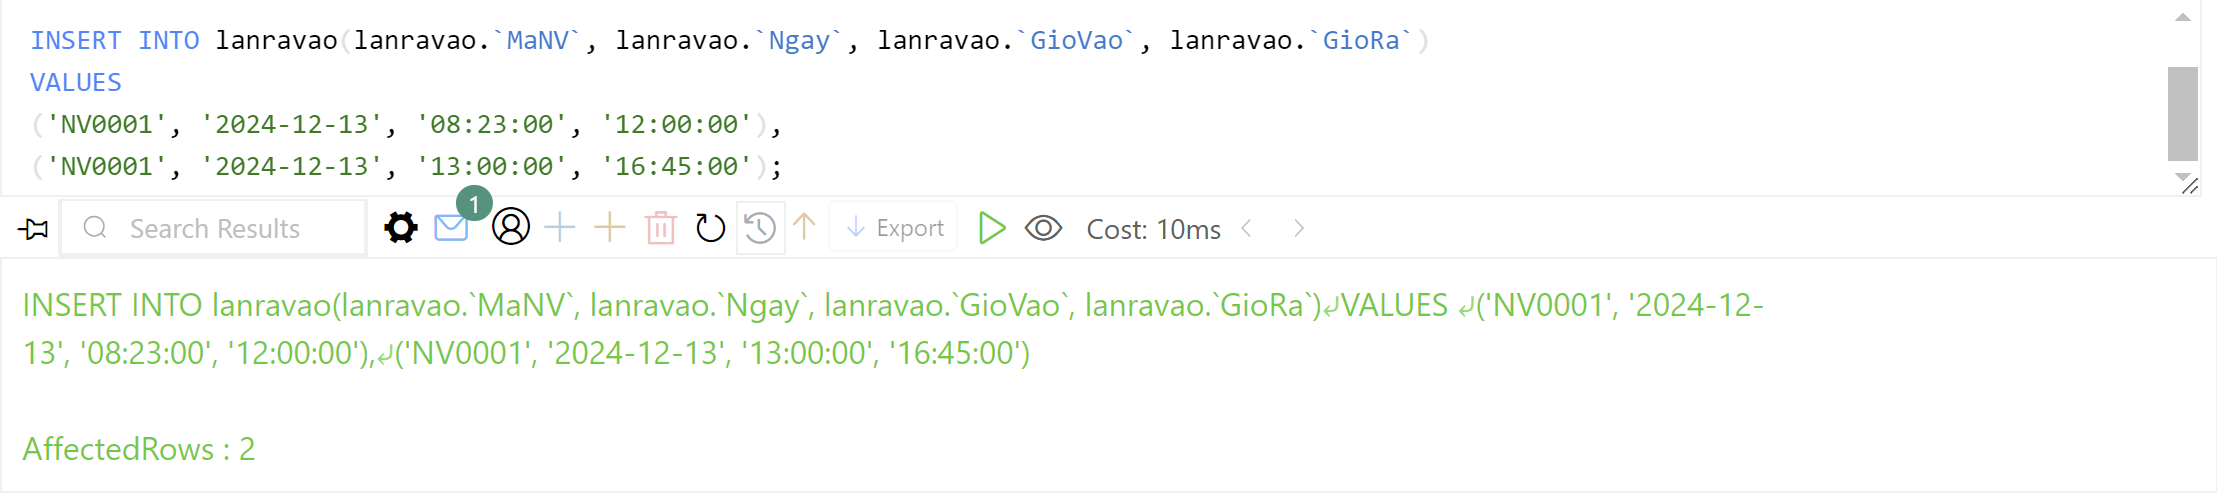
\includegraphics[width=\linewidth]{content/images/trigger_2_2.png}
        \caption{Thực hiện thêm các lần ra vào công ty của nhân viên 'NV0001'}
        \label{fig:trigger_2_2}
    \end{figure}
    \begin{figure}[H]
        \centering
        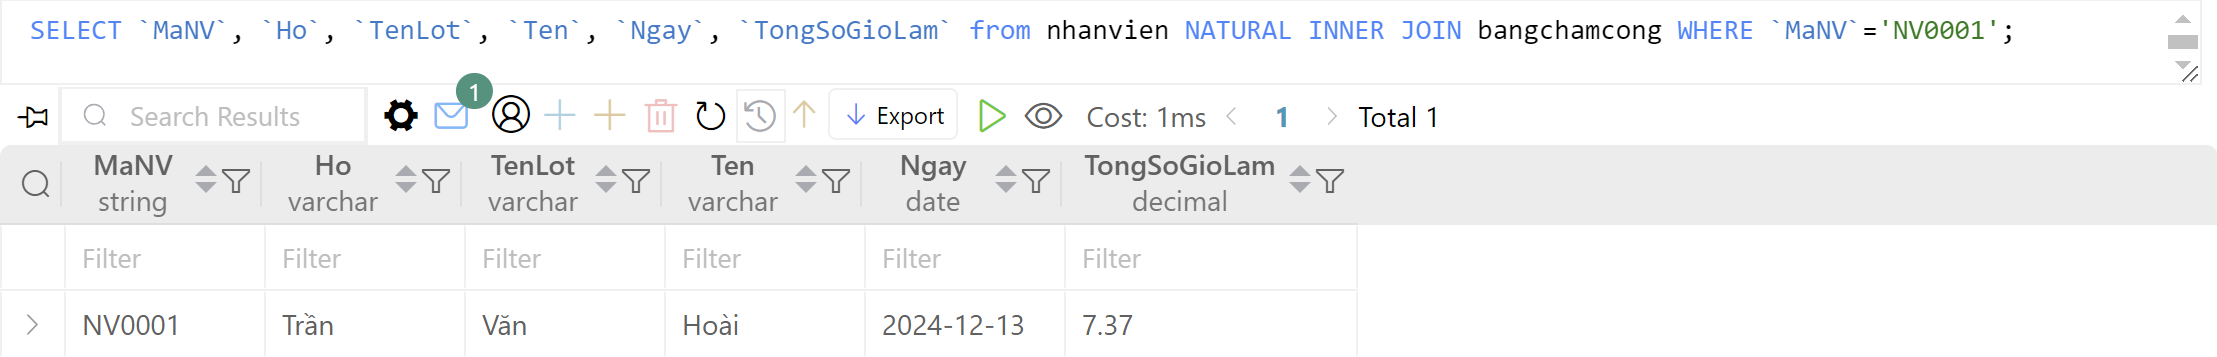
\includegraphics[width=\linewidth]{content/images/trigger_2_3.png}
        \caption{Thông tin của nhân viên 'NV0001', với tổng số giờ làm trong ngày 13/12/2024 đã được cập nhật thành 7.37}
        \label{fig:trigger_2_3}
    \end{figure}
    \item [--] Kiểm tra thao tác cập nhật lần ra vào
    \begin{figure}[H]
        \centering
        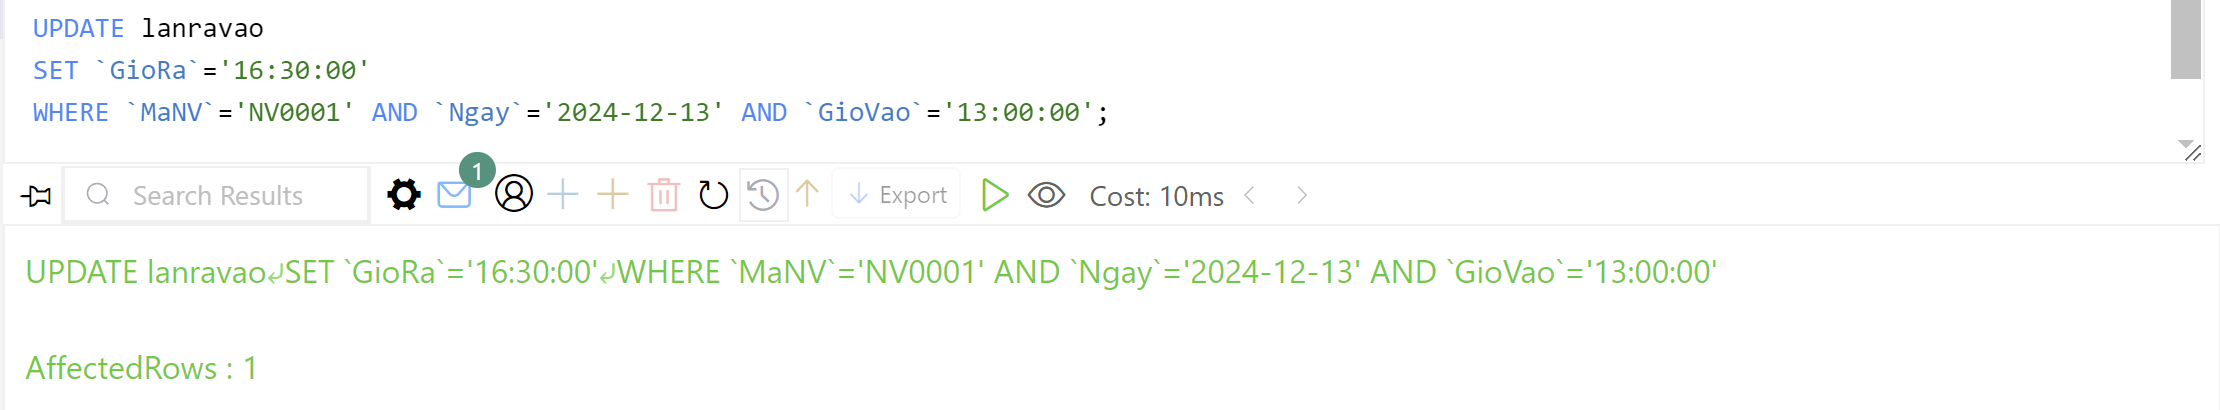
\includegraphics[width=\linewidth]{content/images/trigger_2_4.png}
        \caption{Thực hiện giảm giờ ra của một thực thể trong bảng LanRaVao đi 15 phút}
        \label{fig:trigger_2_4}
    \end{figure}
    \begin{figure}[H]
        \centering
        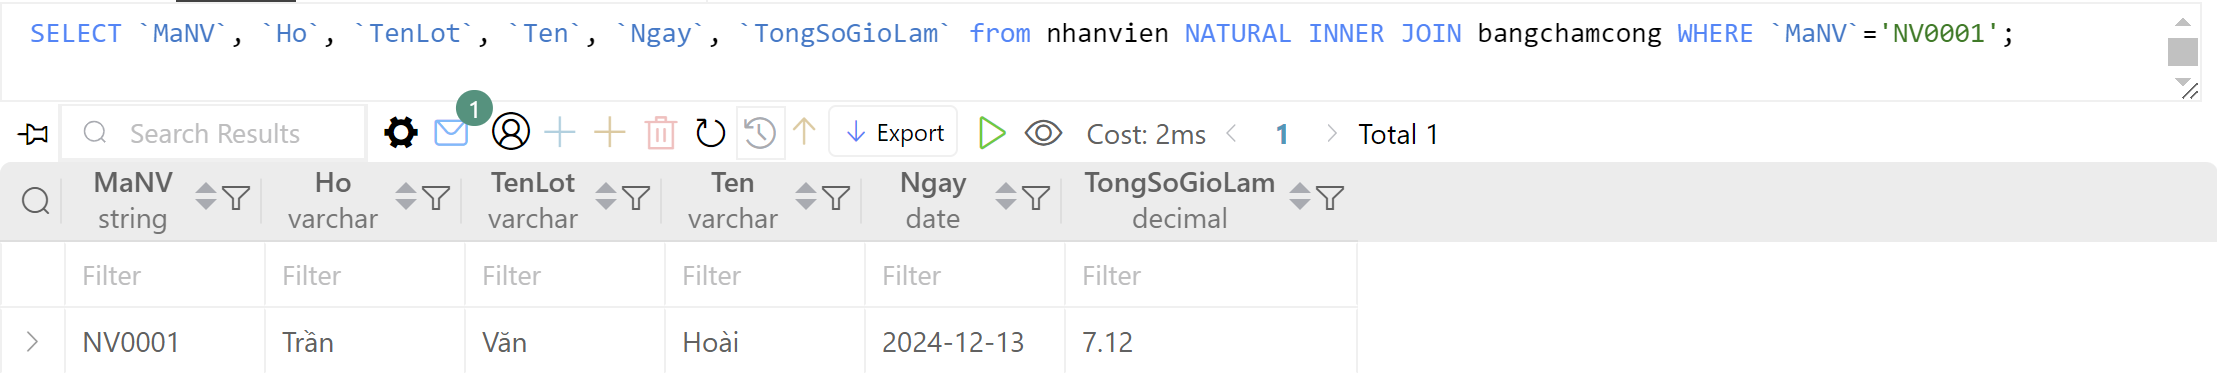
\includegraphics[width=\linewidth]{content/images/trigger_2_5.png}
        \caption{Thông tin của nhân viên 'NV0001', với tổng số giờ làm trong ngày 13/12/2024 đã giảm từ 7.37 xuống 7.12 (giảm 0.25 giờ = 15 phút)}
        \label{fig:trigger_2_5}
    \end{figure}
    \item [--] Kiểm tra thao tác xóa lần ra vào
    \begin{figure}[H]
        \centering
        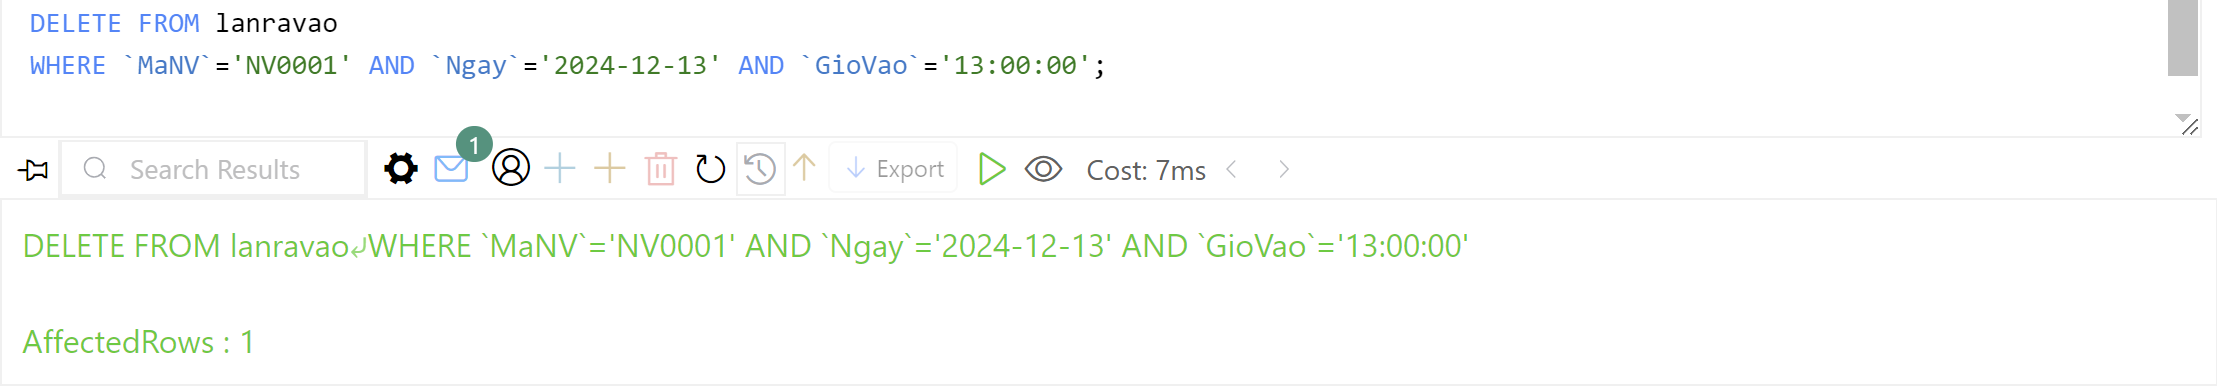
\includegraphics[width=\linewidth]{content/images/trigger_2_6.png}
        \caption{Thực hiện xóa một thực thể trong bảng LanRaVao, tổng thời gian bị xóa là 3 giờ 30 phút}
        \label{fig:trigger_2_6}
    \end{figure}
    \begin{figure}[H]
        \centering
        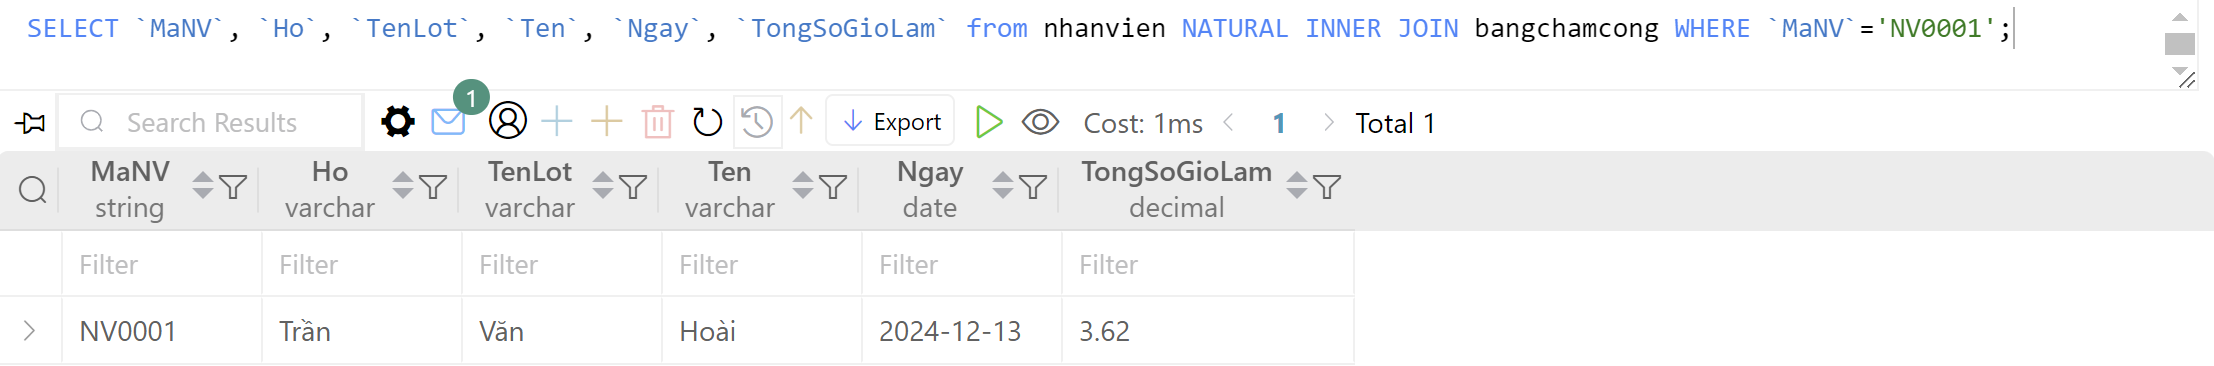
\includegraphics[width=\linewidth]{content/images/trigger_2_7.png}
        \caption{Thông tin của nhân viên 'NV0001', với tổng số giờ làm trong ngày 13/12/2024 đã giảm từ 7.12 xuống 3.62 (giảm 3.5 giờ = 3 giờ 30 phút)}
        \label{fig:trigger_2_7}
    \end{figure}
\end{itemize}

\newpage